We repeat the exact same procedure as in section \ref{sec:eq}, except that we make half of the masses $4$ times as big as the rest. The velocity distributions after equilibrium is reached is plotted in \ref{fig:dist_3}.

\begin{figure}[htb]
	\centering
	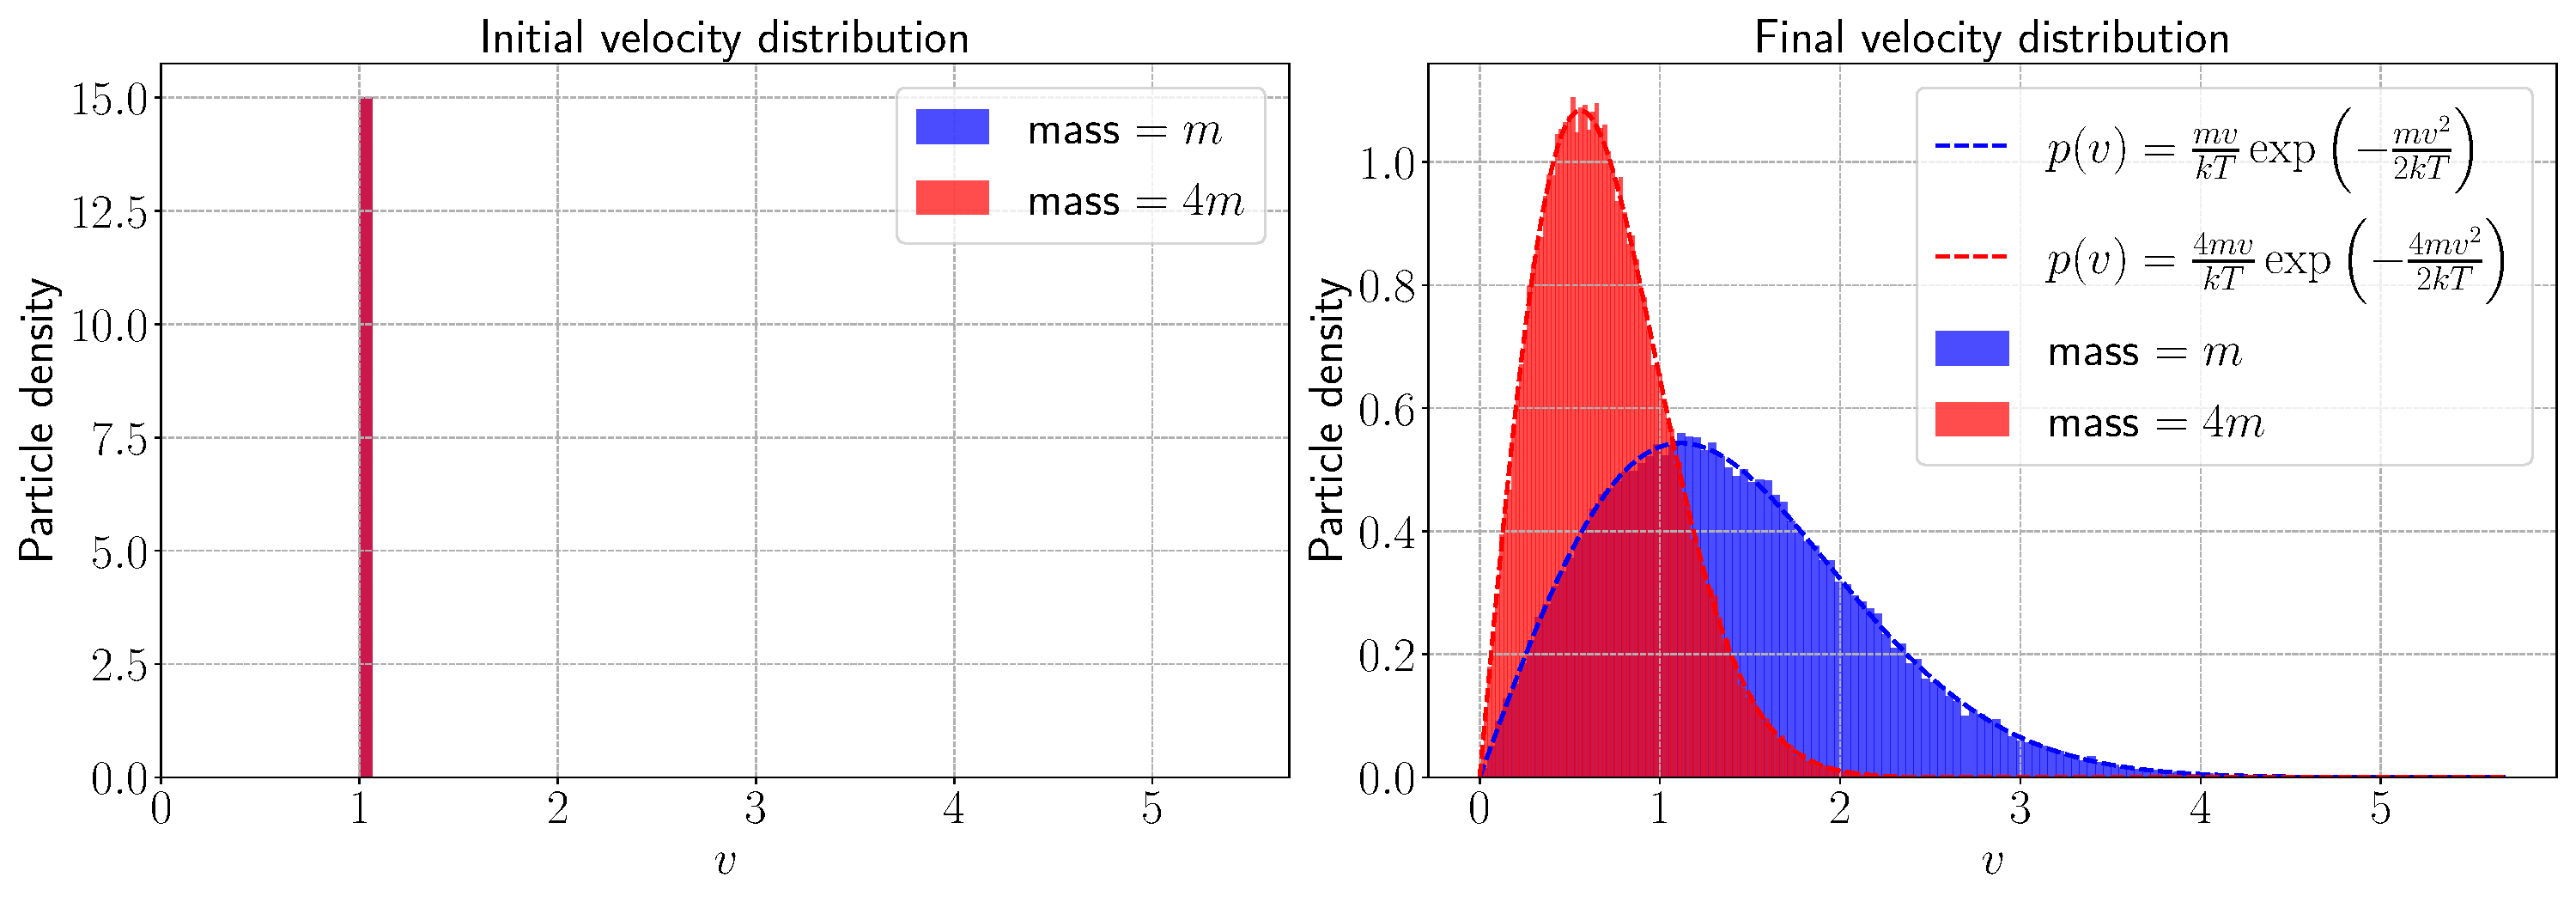
\includegraphics[width=\textwidth]{../fig/distribution_2}
	\caption{Distribution of velocities in a gas of $50000$ particles, here using $112\,00$ samples for each distribution. The red distributions correspond to the heavy particles, while the blue correspond to the lighter particles.}
	\label{fig:dist_3}
\end{figure}

The average speed and kinetic energy is shown in table \ref{tab:averages}. These results suggests that although the masses are different, the mixture of the gases eventually reach equilibrium. The fact that the two gases reaches equilibrium is however most easily seen by actually plotting the time evolution of the average kinetic energy. This is shown in section \ref{sec:mix2}, where we also simulate situations where this is \textit{not} the case.

\begin{table}[htb]
	\centering 
	\caption{Average speed and kinetic energy for the light and heavy particles}
	\begin{tabular}{ccc}
		\toprule
		\textbf{Mass }& \textbf{Average speed} & \textbf{Average kinetic energy} \\
		\midrule
		$m$   & 1.400798 & 12.492590 \\
		$4m$  & 0.701439 & 12.507510 \\
		\bottomrule
	\end{tabular}
	\label{tab:averages}
\end{table}
